\chapter{Теоретическая часть}
\section{Определение $\gamma$-доверительного интервала}

Пусть $X$ --- случайная величина, закон распределения которой известен с точностью до неизвестного параметра $\theta$, $\vec{X}$ --- случайная выборка из генеральной совокупности $X$.

Интервальной оценкой уровня $\gamma \in (0, 1)$ ($\gamma$-интервальной оценкой) параметра $\theta$ называется пара статистик $\underline{\theta}(\vec{X})$ и $\overline{\theta}(\vec{X})$ таких, что
\begin{equation*}
	P\{\theta \in (\underline{\theta}(\vec{X}), \overline{\theta}(\vec{X}))\} = \gamma.
\end{equation*}

$\gamma$-доверительным интервалом для параметра $\theta$ называется интервал $(\underline{\theta}(\vec{x}), \overline{\theta}(\vec{x}))$, являющийся реализацией (выборочным значением) интервальной оценки уровня $\gamma$ для этого параметра.

\section{Формулы для вычисления границ $\gamma$-доверительного интервала}

Пусть $X \sim N(\mu, \sigma^2)$, где $\mu$ и $\sigma^2$ --- неизвестные параметры, $\vec{X}$ --- случайная выборка объема $n$ из генеральной совокупности $X$, $\vec{x}$ --- реализация этой выборки, $\gamma \in (0, 1)$ --- коэфициент доверия.

Для построения $\gamma$-доверительного интервала для $\mu$ используется центральная статистика
\begin{equation*}
	T(\vec{X}, \mu) = \frac{\mu - \overline{X}}{S(\vec{X})}\sqrt{n} \sim St(n - 1).
\end{equation*}

Нижняя и верхняя границы $\gamma$-доверительного интервала для $\mu$ вычисляются по формулам \eqref{eq:lmu} и \eqref{eq:umu}:
\begin{equation}
	\label{eq:lmu}
	\underline{\mu}(\vec{x}) = \overline{x} - t_{\frac{1+\gamma}{2}}^{(n-1)}\sqrt{\frac{S^2(\vec{x})}{n}},
\end{equation}
\begin{equation}
	\label{eq:umu}
	\overline{\mu}(\vec{x}) = \overline{x} + t_{\frac{1+\gamma}{2}}^{(n-1)}\sqrt{\frac{S^2(\vec{x})}{n}},
\end{equation}
\noindent
где $t_{\frac{1+\gamma}{2}}^{(n-1)}$ --- квантиль уровня $\frac{1+\gamma}{2}$ распределения $St(n - 1)$.

Для построения $\gamma$-доверительного интервала для $\sigma^2$ используется центральная статистика
\begin{equation*}
	T(\vec{X}, \sigma^2) = \frac{(n - 1)S^2(\vec{X})}{\sigma^2} \sim \chi^2(n - 1).
\end{equation*}

Нижняя и верхняя границы $\gamma$-доверительного интервала для $\sigma^2$ вычисляются по формулам \eqref{eq:lsigma} и \eqref{eq:usigma}:
\begin{equation}
	\label{eq:lsigma}
	\underline{\sigma}^2(\vec{x}) = S^2(\vec{x})\frac{(n - 1)}{h_{\frac{1+\gamma}{2}}^{(n-1)}},
\end{equation}
\begin{equation}
	\label{eq:usigma}
	\overline{\sigma}^2(\vec{x}) = S^2(\vec{x})\frac{(n - 1)}{h_{\frac{1-\gamma}{2}}^{(n-1)}},
\end{equation}
\noindent
где $h_{\frac{1+\gamma}{2}}^{(n-1)}$ --- квантиль уровня $\frac{1+\gamma}{2}$ распределения $\chi^2(n - 1)$, \\
$h_{\frac{1-\gamma}{2}}^{(n-1)}$ --- квантиль уровня $\frac{1-\gamma}{2}$ распределения $\chi^2(n - 1)$.

\chapter{Практическая часть}
\section{Текст программы}
Текст программы представлен в листинге \ref{prog}.

\begin{lstlisting}[caption={Текст программы}, label={prog}]
X = [-2.54, -0.79, -4.27, -3.09, -3.82, -0.61, -0.64, -1.24, -1.73, -2.91, -1.48, -1.28, -0.37, -1.88, -2.19, -1.61, -1.52, -3.17, -1.36, -3.08, -3.11, -3.07, -1.57, -1.51, -2.37, -0.58, -3.05, -2.93, -1.01, -1.40, -2.06, -3.05, -1.84, -1.24, -1.89, -2.06, -1.59, -2.83, -1.07, -2.96, -3.17, -3.08, -0.49, -3.11, -3.14, -2.30, -3.99, -1.56, -1.28, -3.46, -2.63, -0.82, -2.18, -0.89, -3.08, -1.13, -1.62, -1.06, -2.98, -1.55, -1.49, -1.65, -1.45, -2.29, -0.85, -1.44, -2.87, -2.40, -2.13, -3.52, -1.42, -3.64, -3.47, -2.05, -2.39, -2.07, -0.80, -1.52, -3.92, -2.22, -0.78, -2.60, -1.78, -1.61, -1.65, -2.06, -3.33, -3.41, -1.97, -1.74, -2.04, 0.01, -1.37, -3.15, -2.35, -3.66, -1.79, -2.56, -1.87, -1.06, -0.64, -2.49, -1.85, -1.40, -0.86, -0.17, -0.62, -2.85, -2.12, -1.17, -2.48, -1.65, -3.74, -2.87, -3.15, -1.89, -1.34, -4.33, -0.96, -1.79];
N = length(X);
gamma = 0.9;
alpha = 1 - gamma;
mu_hat_N = mean(X);
S2_N = var(X);
fprintf('Точечная оценка mu: %.4f\n', mu_hat_N);
fprintf('Точечная оценка S^2: %.4f\n', S2_N);
n_range = 2:N;
mu_n = zeros(size(n_range));
mu_low = zeros(size(n_range));
mu_high = zeros(size(n_range));
S2_n = zeros(size(n_range));
S2_low = zeros(size(n_range));
S2_high = zeros(size(n_range));
for i = 1:length(n_range)
    n = n_range(i);
    current_X = X(1:n);
    m_n = mean(current_X);
    s2_n = var(current_X);
    s_n = sqrt(s2_n);
    t_crit = tinv(1 - alpha/2, n - 1);
    chi_low = chi2inv(alpha/2, n - 1);
    chi_high = chi2inv(1 - alpha/2, n - 1);
    mu_n(i) = m_n;
    mu_low(i) = m_n - t_crit * s_n / sqrt(n);
    mu_high(i) = m_n + t_crit * s_n / sqrt(n);
    S2_n(i) = s2_n;
    S2_low(i) = (n - 1) * s2_n / chi_high;
    S2_high(i) = (n - 1) * s2_n / chi_low;
end
S_N = sqrt(S2_N);
avg = mean(X);
t_crit_final = tinv(1 - alpha/2, N - 1);
chi_low_final = chi2inv(alpha/2, N - 1);
chi_high_final = chi2inv(1 - alpha/2, N - 1);
mu_low_final = avg - t_crit_final * S_N / sqrt(N);
mu_high_final = avg + t_crit_final * S_N / sqrt(N);
S2_low_final = (N - 1) * S2_N / chi_high_final;
S2_high_final = (N - 1) * S2_N / chi_low_final;
fprintf('Нижняя граница для mu: %.4f\n', mu_low_final);
fprintf('Верхняя граница для mu: %.4f\n', mu_high_final);
fprintf('Нижняя граница для sigma^2: %.4f\n', S2_low_final);
fprintf('Верхняя граница для sigma^2: %.4f\n', S2_high_final);
figure('Name', 'Оценка MX');
hold on;
plot(n_range, repmat(mu_hat_N, size(n_range)), 'k--', 'LineWidth', 1.5);
plot(n_range, mu_n, 'k-', 'LineWidth', 1.5);
plot(n_range, mu_high, '-', 'Color', [0.5 0.5 1], 'LineWidth', 1.2);
plot(n_range, mu_low, '-', 'Color', [0.5 0.5 1], 'LineWidth', 1.2);
title('Доверительный интервал для MX');
xlabel('Объем выборки n');
ylabel('y');
legend('$\hat{\mu}(\vec{x}_N)$', '$\hat{\mu}(\vec{x}_n)$', '$\overline{\mu}(\vec{x}_n)$', '$\underline{\mu}(\vec{x}_n)$', 'Location', 'best', 'Interpreter', 'latex', 'FontSize', 14);
grid on;
hold off;
figure('Name', 'Оценка DX');
hold on;
plot(n_range, repmat(S2_N, size(n_range)), 'k--', 'LineWidth', 1.5);
plot(n_range, S2_n, 'k-', 'LineWidth', 1.5);
plot(n_range, S2_high, '-', 'Color', [0.5 0.5 1], 'LineWidth', 1.2);
plot(n_range, S2_low, '-', 'Color', [0.5 0.5 1], 'LineWidth', 1.2);
title('Доверительный интервал для DX');
xlabel('Объем выборки n');
ylabel('z');
legend('$S^2(\vec{x}_N)$', '$S^2(\vec{x}_n)$', '$\overline{\sigma}^2(\vec{x}_n)$', '$\underline{\sigma}^2(\vec{x}_n)$', 'Location', 'best', 'Interpreter', 'latex', 'FontSize', 14);
grid on;
hold off;
idx_5 = n_range >= 5;
n_range_5 = n_range(idx_5);
S2_n_5 = S2_n(idx_5);
S2_high_5 = S2_high(idx_5);
S2_low_5 = S2_low(idx_5);
figure('Name', 'Оценка DX (n >= 5)');
hold on;
plot(n_range_5, repmat(S2_N, size(n_range_5)), 'k--', 'LineWidth', 1.5);
plot(n_range_5, S2_n_5, 'k-', 'LineWidth', 1.5);
plot(n_range_5, S2_high_5, '-', 'Color', [0.5 0.5 1], 'LineWidth', 1.2);
plot(n_range_5, S2_low_5, '-', 'Color', [0.5 0.5 1], 'LineWidth', 1.2);
title('Доверительный интервал для DX при n \geq 5');
xlabel('Объем выборки n');
ylabel('z');
legend('$S^2(\vec{x}_N)$', '$S^2(\vec{x}_n)$', '$\overline{\sigma}^2(\vec{x}_n)$', '$\underline{\sigma}^2(\vec{x}_n)$', 'Location', 'best', 'Interpreter', 'latex', 'FontSize', 14);
grid on;
hold off;
\end{lstlisting}

\clearpage

\section{Результаты расчетов}
Результаты расчетов для выборки из индивидуального варианта при $\gamma = 0.9$ приведены на формулах \eqref{eq:res_mu}, \eqref{eq:res_s}, \eqref{eq:res_lmu}, \eqref{eq:res_hmu}, \eqref{eq:res_lsigma}, \eqref{eq:res_hsigma}.

\begin{equation}
	\label{eq:res_mu}
	\hat{\mu}(\vec{x}_N) = -2.0585
\end{equation}
\begin{equation}
	\label{eq:res_s}
	S^2(\vec{x}_N) = 0.9440
\end{equation}
\begin{equation}
	\label{eq:res_lmu}
	\underline{\mu}(\vec{x}_n) = -2.2055
\end{equation}
\begin{equation}
	\label{eq:res_hmu}
	\overline{\mu}(\vec{x}_n) = -1.9115
\end{equation}
\begin{equation}
	\label{eq:res_lsigma}
	\underline{\sigma}^2(\vec{x}_n) = 0.7723
\end{equation}
\begin{equation}
	\label{eq:res_hsigma}
	\overline{\sigma}^2(\vec{x}_n) = 1.1848
\end{equation}

На рисунке \ref{image:graph1} представлена прямая $y = \hat{\mu}(\vec{x}_N)$, а также графики функций $y = \hat{\mu}(\vec{x}_n)$, $y = \overline{\mu}(\vec{x}_n)$, $y = \underline{\mu}(\vec{x}_n)$ как функций объема $n$ выборки, где $n$ изменяется от 1 до $N$.
\begin{figure}[h]
	\centering{
		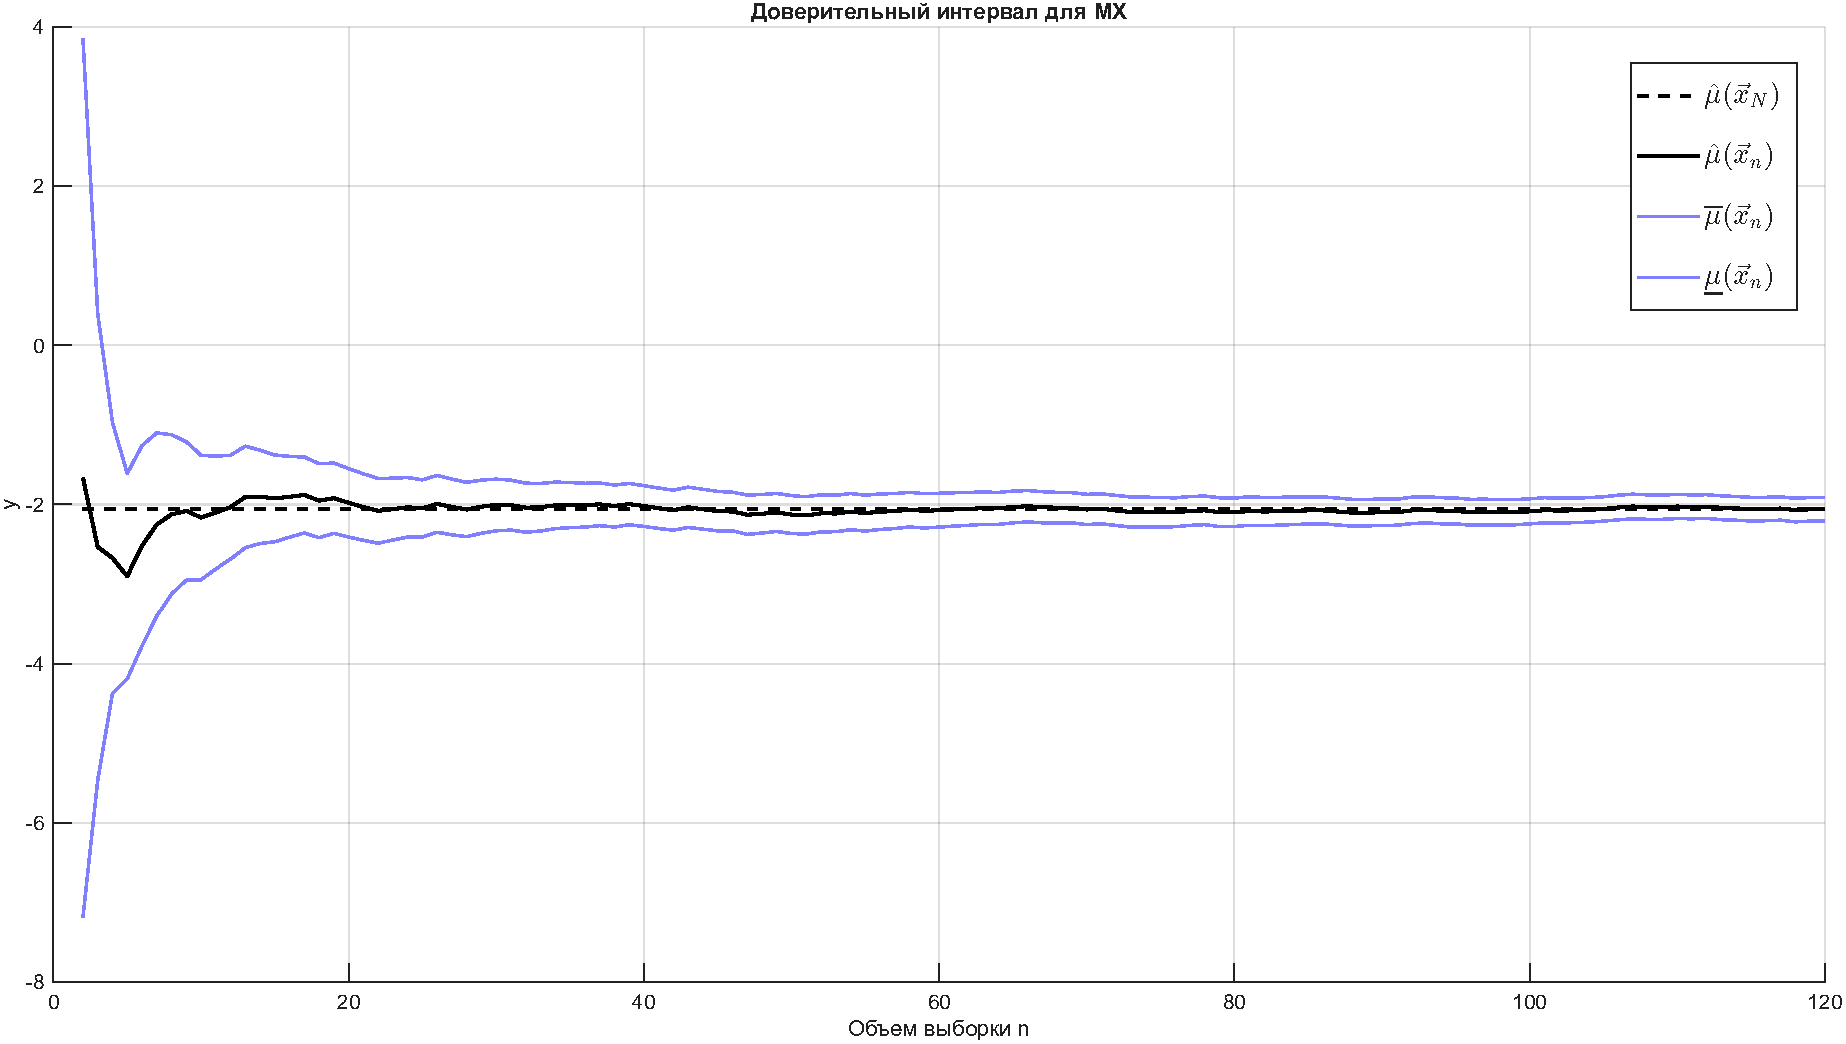
\includegraphics[scale=0.5]{./img/MX.pdf}
		\caption{Графики функций для MX}
		\label{image:graph1}
	}
\end{figure}

\clearpage

На рисунке \ref{image:graph2} представлена прямая $y = S^2(\vec{x}_N)$, а также графики функций $y = S^2(\vec{x}_n)$, $y = \overline{\sigma}^2(\vec{x}_n)$, $y = \underline{\sigma}^2(\vec{x}_n)$ как функций объема $n$ выборки, где $n$ изменяется от 2 до $N$.
\begin{figure}[h]
	\centering{
		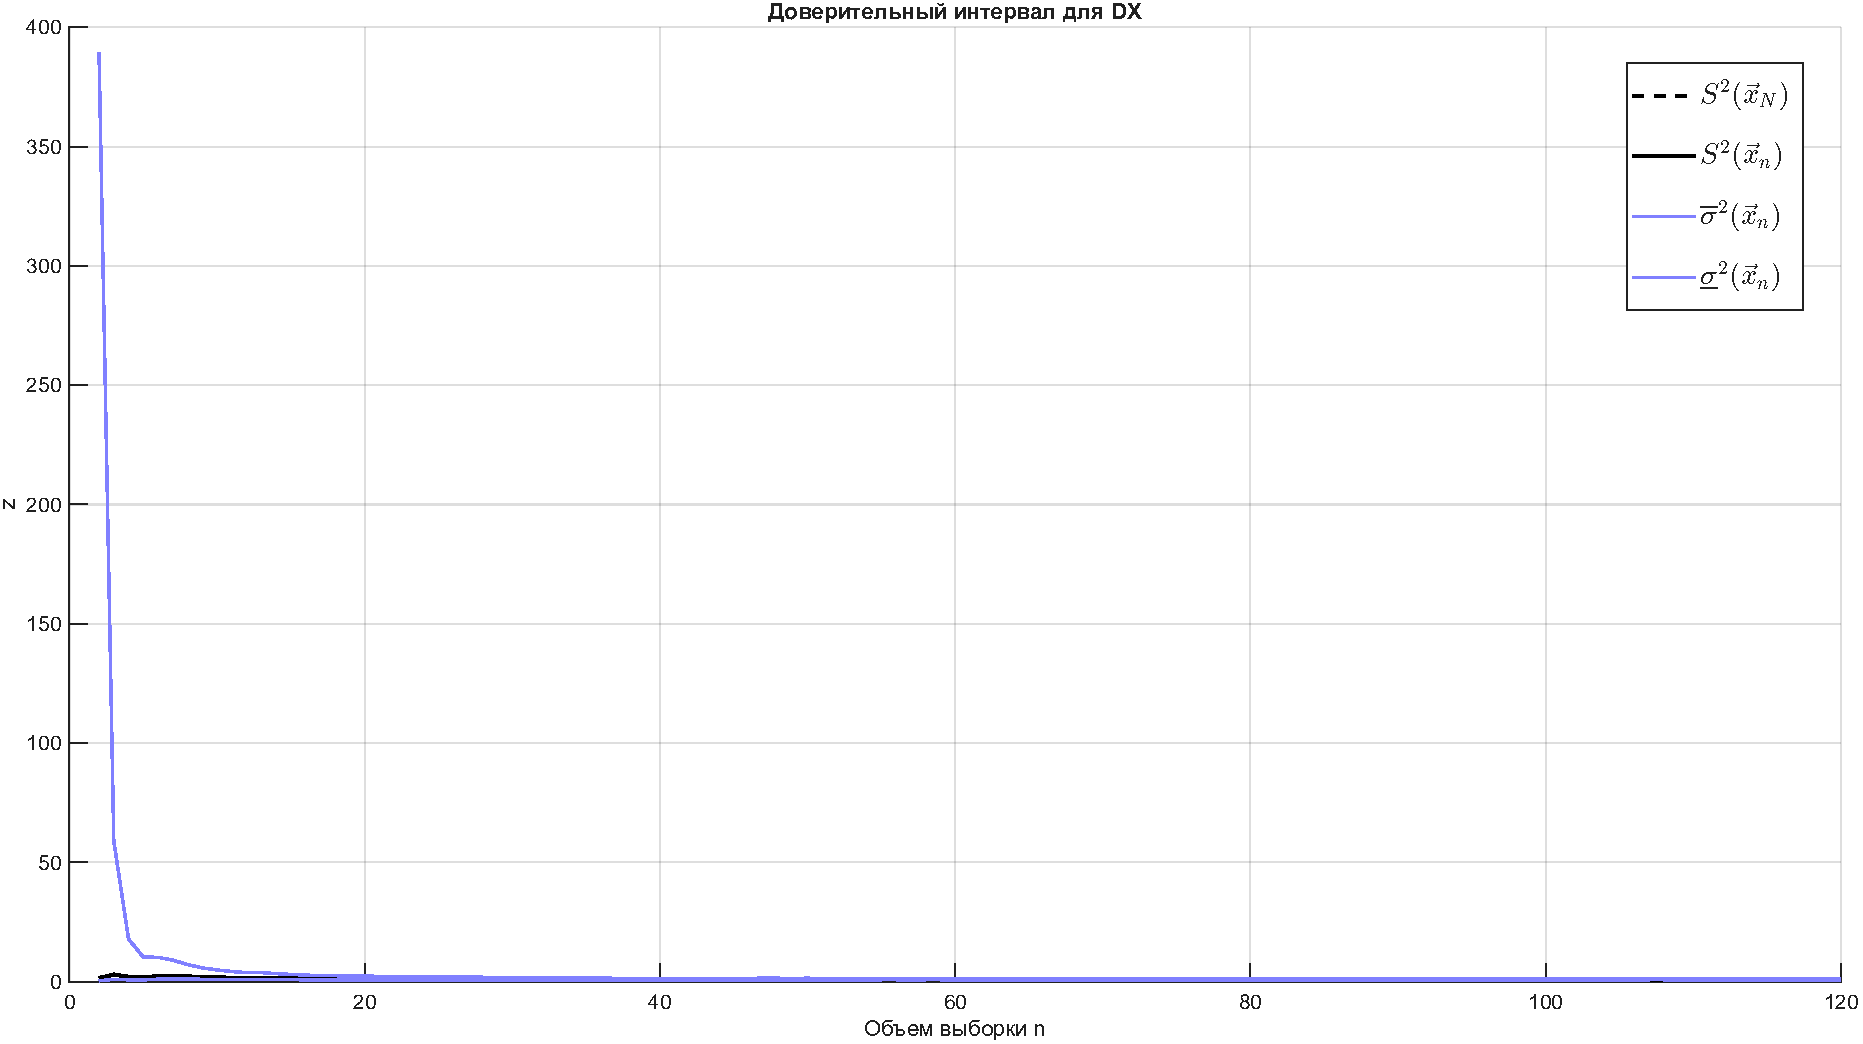
\includegraphics[scale=0.5]{./img/DX.pdf}
		\caption{Графики функций для DX}
		\label{image:graph2}
	}
\end{figure}
